\documentclass[
	draft=false,
	paper=a4,
	twoside=false,
	fontsize=11pt,
	headsepline,
	BCOR10mm,
	DIV11
]{scrbook}
\usepackage[ngerman,english]{babel}
%% see http://www.tex.ac.uk/cgi-bin/texfaq2html?label=uselmfonts
\usepackage[T1]{fontenc}
%\usepackage[utf8]{inputenc}
\usepackage[latin1]{inputenc}
\usepackage{ngerman}
\usepackage{lmodern}
\usepackage{libertine}
\usepackage{pifont}
\usepackage{microtype}
\usepackage{textcomp}
\usepackage[german,refpage]{nomencl}
\usepackage{setspace}
\usepackage{makeidx}
\usepackage{listings}
\usepackage{natbib}
\usepackage[ngerman,colorlinks=true]{hyperref}
\usepackage{soul}
\usepackage{hawstyle}
\usepackage{graphicx}
%%\usepackage[texencoding=utf8, backend=biber, style=din1505, block=none, mincrossrefs=9999]{biblatex}

%% define some colors
\colorlet{BackgroundColor}{gray!20}
\colorlet{KeywordColor}{blue}
\colorlet{CommentColor}{black!60}
%% for tables
\colorlet{HeadColor}{gray!60}
\colorlet{Color1}{blue!10}
\colorlet{Color2}{white}

%% configure colors
\HAWifprinter{
	\colorlet{BackgroundColor}{gray!20}
	\colorlet{KeywordColor}{black}
	\colorlet{CommentColor}{gray}
	% for tables
	\colorlet{HeadColor}{gray!60}
	\colorlet{Color1}{gray!40}
	\colorlet{Color2}{white}
}{}
\lstset{
	numbers=left,
	numberstyle=\tiny,
	stepnumber=1,
	numbersep=5pt,
	basicstyle=\ttfamily\small,
	keywordstyle=\color{KeywordColor}\bfseries,
	identifierstyle=\color{black},
	commentstyle=\color{CommentColor},
	backgroundcolor=\color{BackgroundColor},
	captionpos=b,
	fontadjust=true
}
\lstset{
	escapeinside={(*@}{@*)}, % used to enter latex code inside listings
	morekeywords={uint32_t, int32_t}
}
\ifpdfoutput{
	\hypersetup{bookmarksopen=false,bookmarksnumbered,linktocpage}
}{}

%% more fancy C++
\DeclareRobustCommand{\cxx}{C\raisebox{0.25ex}{{\scriptsize +\kern-0.25ex +}}}

\clubpenalty=10000
\widowpenalty=10000
\displaywidowpenalty=10000

% unknown hyphenations
\hyphenation{
}

%% recalculate text area
\typearea[current]{last}

\makeindex
\makenomenclature

\begin{document}
	\selectlanguage{ngerman}
	
	%%%%%
	%% customize (see readme.pdf for supported values)
	\HAWThesisProperties{
		Author={Lars Nielsen},
		Title={Partikelsysteme},
		EnglishTitle={Particle Systems},
		ThesisType={Projektarbeit},
		ExaminationType={Projektarbeit},
		DegreeProgramme={Bachelor of Science Angewandte Informatik},
		ThesisExperts={Prof. Dr. Jenke},
		ReleaseDate={16. M�rz 2017}
	}
	
	\frontmatter
	\maketitle
	\onehalfspacing
	
	%% note: this is one command on multiple lines
	\HAWAbstractPage
	%% German abstract
	{Partikelsysteme, Partikel}%
	{Dieses Dokument fasst die Erkenntnisse und Techniken zusammen, die zur Entwicklung eines Partikelsystems im Rahmen der Projektarbeit f�r das Wahlpflichtfach Computergraphik angewendet wurden.}
	%% English abstract
	{particle systems, particle}%
	{This document summarizes the findings and techniques that were used for developing a particle system within the scope of the project realized for Computergraphik.}
	
	\newpage
	\singlespacing
	
	\tableofcontents
	\newpage
	%% enable if these lists should be shown on their own page
	%%\listoftables
	%%\listoffigures
	%%\lstlistoflistings
	
	%% main
	\mainmatter
	\onehalfspacing
	
	\chapter{Einleitung} \label{introduction}
\textmd{Partikelsysteme werden in der Computergraphik zur Simulation von unterschiedlichsten undeutlichen Objekten eingesetzt. Ein Partikelsystem besteht dabei aus einer Vielzahl von einzelnen Partikeln, die zusammen ein Ph�nomen wie zum Beispiel Feuer, Regen oder Schnee darstellen.}

\textmd{\\Ihren Ursprung haben Partikelsysteme aus dem Film Star Trek II: The Wrath of Khan. Der Forscher William T. Reeves von Lucasfilm Ltd. entwickelte 1982 das erste Partikelsystem f�r den Genesis Effect, vgl. \cite{natureofcode2012}.}

\section{Aufgabenstellung} \label{problem}
\textmd{Diese Projektarbeit befasst sich mit der Erstellung eines Partikelsystems. Dabei sollen sowohl die Grundlagen wie die Darstellung und Repr�sentation von Partikeln und Partikelsystemen ber�cksichtigt werden, als auch fortgeschrittenere Themen wie Performance und der Umgang mit Transparenz.}

\section{Struktur der Arbeit} \label{structure}
\textmd{Diese Arbeit besteht aus drei Teilen. Im n�chsten Kapitel werden zun�chst Partikelsysteme generell erkl�rt und worauf bei ihrer Implementation geachtet werden muss. Das dritte Kapitel besch�ftigt sich mit der Implementation einer API f�r Partikelsysteme in dem Framework aus dem Wahlpflichtfach Computergrafik. In dem letzten Kapitel werden Erkenntnisse und Probleme aus der Arbeit dargestellt und zuletzt ein Ausblick gegeben, welche weiteren M�glichkeiten Partikelsysteme bieten.}

	\chapter{Partikelsysteme} \label{particlesystems}
\textmd{\textquotedblleft A particle system is a collection of many many minute particles that together represent a fuzzy object. Over a period of time, particles are generated into a system, move and change from within the system, and die from the system.\textquotedblright\quad\cite[S. 92]{reeves1983}}

\textmd{\\Partikelsysteme bestehen also aus einer Vielzahl von einzelnen Partikeln die durch das Partikelsystem verwaltet werden. Ein Partikel zeichnet sich haupts�chlich dadurch aus, dass er eine beschr�nkte Lebensdauer hat. Abh�ngig von der Lebenszeit k�nnen dann weitere Eigenschaften modelliert werden, wie zum Beispiel Geschwindigkeit, Beschleunigung, Masse oder Farbe.}

\textmd{\\�ber die Lebenszeit eines Partikelsystems werden st�ndig Partikel hinzugef�gt und entfernt. Je nach Art und Lebensdauer des Partikelsystems k�nnen dadurch sehr viele Partikel erzeugt werden, was bei der Implementation ber�cksichtigt werden muss. Au�erdem muss zwischen Partikelsystemen unterschieden werden, die dauerhaft leben und jenen die ein begrenztes Dasein fristen.}


	\chapter{Implementation} \label{implementation}
\textmd{In diesem Kapitel wird die Implementation des Partikelsystems aus dem Projekt erl�utert. Dabei wird auf die Techniken eingegangen, die zur Realisierung des Partikelsystems eingesetzt wurden.}

\section{Datenstrukturen} \label{datastructures}
\textmd{Dieser Abschnitt beschreibt die angelegten Datenstrukturen und Algorithmen um Partikelsysteme zu realisieren und zu verwalten. Davon abgegrenzt ist die Darstellung eines Partikelsystems die in Abschnitt \ref{rendering} beschrieben wird.}

\textmd{\\Partikel wurden mit der Klasse Particle modelliert. Sie verf�gt �ber eine Lebenszeit, physikalische Eigenschaften wie Position, Geschwindigkeit und Beschleunigung, sowie Farbe. Eine update-Funktion sorgt f�r das Aktualisieren der Eigenschaften �ber den Lebenszyklus des Partikels. Getter und Setter erm�glichen den Zugriff auf ihre Eigenschaften, wobei die Setter eher nicht direkt verwendet werden sollten. F�r das Setzen der Eigenschaften gibt es mit Particle.Builder eine Klasse �ber die Partikel konfiguriert und anschlie�end erzeugt werden k�nnen.}

\textmd{\\Partikelsysteme sind durch die Klasse ParticleSystem modelliert. Ein Partikelsystem verwaltet alle seine zugeh�rigen Partikel. Es erh�lt bei der Instanziierung einen Particle.Builder �bergeben, anhand dessen Konfiguration die Partikel des Partikelsystems erzeugt werden.}
\textmd{\\Das Partikelsystem hat eine update-Methode, die das Erzeugen neuer Partikel sowie das Aktualisieren und Sterben bestehender Partikel umsetzt. Daf�r wird anhand der Systemzeit berechnet wie viele Millisekunden seit dem letzten update-Aufruf vergangen sind und als zeitliches Delta verwendet. Daraus wird wiederum die Ver�nderung der Partikeleigenschaften berechnet, wie zum Beispiel die neue Position oder Farbe.}
\textmd{\\An einem Partikelsystem kann festgelegt werden, wie viele Partikel maximal gleichzeitig existieren und wie viele Partikel pro Sekunde erzeugt werden k�nnen. Um einen stetigen Partikelfluss zu gew�hrleisten hat sich die Faustregel in Formel \ref{emissionrate} durchgesetzt, vgl. \cite[Abschnitt Emission Rate]{greer2012}.}
\begin{align}
	Emissionsrate = \frac{maxPartikel}{Lebenszeit_{Partikel}}
	\label{emissionrate}
\end{align}

\textmd{\\Mit ParticleSystemManager gibt es eine Klasse die alle erzeugten Partikelsysteme verwalten kann, vgl. \cite[Kapitel 4.5 A System of Systems]{natureofcode2012}, \cite[Kapitel Systems of particle systems]{khan}. Der ParticleSystemManager bietet Funktionen zum Hinzuf�gen und Entfernen von Partikelsystemen an. Weiterhin k�mmert er sich um das Updaten der registrierten Partikelsysteme und entfernt sie wenn sie tot sind, vgl. \cite[S. 3]{gamasutra2000}. Weiteres dazu kann in dem Kapitel \ref{lifecyclemanagement} zum Lebenszyklusmanagement nachgelesen werden.}
\textmd{Um auf Ereignisse des ParticleSystemManagers reagieren zu k�nnen, k�nnen entsprechend des Listener-Patterns Listener registriert werden. Zur Zeit implementierte Ereignisse sind das Hinzuf�gen, das Sterben und das Entfernen von Partikelsystemen.}

\section{Lebenszyklusmanagement} \label{lifecyclemanagement}
\textmd{In diesem Abschnitt wird zun�chst das Lebenszyklusmanagement von Partikeln und danach das Lebenszyklusmanagement von Partikelsystemen beschrieben.}

\textmd{\\Partikelsysteme erzeugen st�ndig neue Partikel und bestehende Partikel sterben. In der einfachsten Implementation k�nnte eine Liste der lebendigen Partikel gef�hrt werden und die sterbenden Partikel aus der Liste entfernt werden. Das f�hrt dazu, dass sehr viele Objekte erzeugt und wieder vom Garbage-Collector aufger�umt werden m�ssen. Dabei sind sowohl die Objekt-Erzeugung und -Zerst�rung relativ zeit-aufw�ndige Vorg�nge. Indem die gestorbenen Partikel nicht verworfen sondern wiederverwendet werden, kann der Overhead f�r die Objekt-Erzeugung und -Zerst�rung auf das N�tigste reduziert werden, vgl. \cite[S. 1]{gamasutra2000}.}

\textmd{\\In der Implementation aus dieser Arbeit gibt es hierf�r zwei Sammlungen, eine f�r lebendige Partikel (lifeParticles) und eine f�r tote Partikel (deadParticles). Nur die Partikel in lifeParticles erhalten Updates. Die Summe der Partikel aus beiden Sammlungen darf die Maximalzahl an Partikeln nicht �bersteigen, die an dem Partikelsystem festgelegt wurde. Sollen neue Partikel erzeugt werden, so werden Partikel aus deadParticles anhand des Particle.Builders zur�ckgesetzt und nach lifeParticles verschoben. Stirbt ein Partikel wird er in seinem aktuellen Zustand von lifeParticles nach deadParticles verschoben und erh�lt so keine Updates mehr.}
\textmd{\\Es gibt alternative Implementationen, die mit nur einer Liste auskommen. Die lebendigen Partikel werden hierbei vorne und die toten Partikel hinten einsortiert, vgl. \cite[Abschnitt How the Particle Pool Works]{greer2012}, \cite[Kapitel 4.3 The ArrayList]{natureofcode2012}, \cite[Kapitel A particle system]{khan}. Ich habe mich hier f�r die Variante mit den zwei Sammlungen entschieden, da ich so eine komplette Sammlung iterieren kann und nicht darauf achten muss, sie nur bis zu einem Teil zu iterieren. Das Sortieren wird durch das verschieben in die jeweils andere Sammlung umgesetzt. Da hier aber zwei Sammlungen eingesetzt werden ist mein Ansatz an der Stelle geringf�gig speicherintensiver.}

\textmd{\\So wie Partikel sterben, k�nnen auch Partikelsysteme sterben. Es gibt Partikelsysteme die in einer Endlosschleife Partikel erzeugen, wie zum Beispiel Feuer und welche die nur �ber eine begrenzte Zeit Partikel erzeugen, wie bei einer Explosion. Letztere sterben nachdem ihre Partikel ihre Lebenszeit vollendet haben und keine weiteren Partikel mehr erzeugt werden sollen. Um keine Updates auf Partikelsysteme zu verschwenden die nicht mehr angezeigt werden sollen, k�mmert sich der ParticleSystemManager darum diese zu entfernen, vgl. \cite[S. 3]{gamasutra2000}. Durch das in Abschnitt \ref{datastructures} erw�hnte Listener-Pattern k�nnen Softwarekomponenten �ber den Tod eines Partikelsystems benachrichtigt werden, die nun gegebenenfalls Referenzen auf das Partikelsystem invalidieren k�nnen.}

\section{Kr�fte} \label{forces}
\textmd{Dieser Abschnitt erkl�rt die Implementation von physikalischen Kr�ften innerhalb des Projekts.}

\textmd{\\Partikel die sich bewegen k�nnen, verf�gen in der Regel �ber die physikalischen Eigenschaften Position, Geschwindigkeit und Beschleunigungm, vgl. \cite[Kapitel 4.2 A Single Particle]{natureofcode2012}. In jedem Update-Zyklus wird die n�chsth�here Eigenschaft auf die Aktuelle addiert. So wird die Beschleunigung auf die Geschwindigkeit und die Geschwindigkeit auf die Position addiert, was es den Partikeln erm�glicht sich zu bewegen. �nderungen an der Beschleunigung pflanzen sich so fort und nehmen Einfluss auf die Position.}

\textmd{\\Um Partikel physikalisch korrekt zu bewegen und Kr�fte wie Wind und Schwerkraft zu modellieren bedarf es noch der Eigenschaft Masse. Die Masse hat Einfluss darauf, wie stark Kr�fte auf das Partikel einwirken. Schwerkraft unterscheidet sich hier von normalen Kr�ften, insofern die Masse keine Auswirkung auf die Schwerkraft hat, vgl. \cite[Kapitel Particle systems with forces, Abschnitt Adding Gravity]{khan}.}

\textmd{\\In der Implementation werden Kr�fte dem Partikelsystem per apply- bzw. removeForce hinzugef�gt bzw. entfernt. Das Partikelsystem addiert alle Kr�fte die angewendet werden sollen auf zu der sogenannten Netforce, vgl. \cite[Kapitel Understanding net forces]{pixar}. Die Netforce wird nun bei jedem Update-Zyklus auf jeden Partikel angewendet. Hier wird die Netforce mit der Masse des Partikels verrechnet und das Ergebnis daraus ist die Beschleunigung des Partikels f�r diesen Update-Zyklus. Nachdem die Beschleunigung auf die Geschwindigkeit verrechnet wurde, wird sie wieder zur�ck auf 0 gesetzt.}

\section{Darstellung} \label{rendering}
\textmd{In diesem Abschnitt wird die Darstellung der Partikelsysteme beschrieben. Das Projekt verwendet den aus dem Praktikum bekannten Szenengraphen. Die Einbindung eines Partikelsystems in den Szenengraphen wird mit einem ParticleSystemNode realisiert. Dieser erh�lt bei seiner Erzeugung das Partikelsystem das er darstellen soll. Ab der Einbindung in den Szenengraphen ist der ParticleSystemNode f�r das Aktualisieren und Zeichnen des Partikelsystems zust�ndig. Zum Zeichnen wird ein VertexBufferObject der einzelnen Partikel erzeugt und OpenGL �bergeben. Zur fl�ssigen Darstellung des Partikelsystems geschieht das in jedem Renderzyklus. Um die H�ufigkeit des Renderzyklus festzulegen, kann �ber die Klasse ParticleSystemShowcaseScene eine gew�nschte Frames-Per-Second-Rate angegeben werden.}

\textmd{\\Die einzelnen Partikel werden als einfache, farbige Punkte gezeichnet. Sie k�nnen �ber die Zeit ausgeblendet werden, was in OpenGL zu Problemen mit der Transparenz f�hrt. Der n�chste Abschnitt beschreibt das Problem und den Umgang mit der Transparenz in OpenGL.}

\section{Transparenz} \label{transparency}
\textmd{Dieser Abschnitt behandelt den Umgang mit Transparenz in der Darstellung der einzelnen Partikel. Standardm��ig werden die Partikel ohne eine bestimmte Sortierung gezeichnet. Das sorgt in OpenGL daf�r, dass Transparenz nicht richtig dargestellt werden kann. Wenn ein transparentes Objekt das n�her zur Kamera ist zuerst gezeichnet wird und danach eines das weiter hinten ist, so werden die Pixel des ersten Objekts nicht mehr angepasst. F�r ein Partikelsystem mit Transparenz sieht das aus wie in Abbildung \ref{transparency-no-btf}. In der Abbildung k�nnen dunkle Partikel beobachtet werden, die transparent sein sollten.}
\begin{figure}[h]
	\begin{center}
		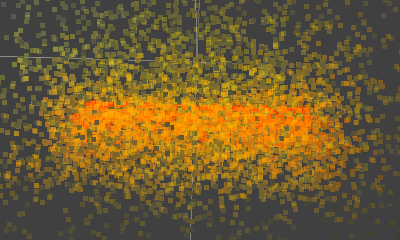
\includegraphics[width=25em]{img/transparency_no_back-to-front_ordering.png}
		\caption{Partikelsystem ohne Back-to-Front-Sortierung}
		\label{transparency-no-btf}
	\end{center}
\end{figure}
\textmd{\\Um die Transparenz korrekt darzustellen wurde eine Back-to-Front-Sortierung unter Zuhilfenahme der Binary-Space-Partition berechnet. Bei der Binary-Space-Partition werden die Partikel r�umlich durch Hyperebenen in einer Baumstruktur getrennt, vgl. \cite[Folie 26]{jenke2016}. Jeder Partikel befindet sich dann entweder vor oder hinter einer Hyperebene, bei der er einsortiert wurde. Betrachtet man nun einen Sichtpunkt, so kann anhand der Hyperebenen die Back-to-Front-Sortierung ermittelt werden, vgl. \cite[Folie 32]{jenke2016}.}
\textmd{\\Die Back-to-Front-Sortierung wiederum ist wichtig um die Partikel in der richtigen Reihenfolge zu zeichnen, sodass OpenGL die Transparenz korrekt darstellt. In der Darstellung des Beispiels aus Abbildung \ref{transparency-no-btf} mit Back-to-Front-Sortierung (siehe Abbildung \ref{transparency-with-btf}) fallen nun keine dunklen Partikel mehr auf.}
\begin{figure}[h]
	\begin{center}
		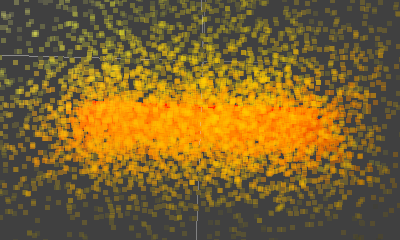
\includegraphics[width=25em]{img/transparency_with_back-to-front_ordering.png}
		\caption{Partikelsystem mit Back-to-Front-Sortierung}
		\label{transparency-with-btf}
	\end{center}
\end{figure}
\textmd{\\\\Es sollte erw�hnt werden, dass die Back-to-Front-Sortierung insbesondere bei einer gro�en Anzahl von Partikeln gewisse Performance-Einbu�en mit sich f�hrt. W�hrend ein Partikelsystem mit 10.000 Partikeln ohne Back-to-Front-Sortierung in meinen Tests mit einer Bildrate von 30 Frames-per-Second gerendert werden kann, so f�llt die Bildrate mit Back-to-Front-Sortierung in dem Szenario auf 10 Frames-per-Second.}
	\chapter{Zusammenfassung und Erkenntnisse} \label{summary}
\textmd{In diesem Kapitel werden Erkenntnisse widergespiegelt, die w�hrend der Implementation des Partikelsystems in dem Projekt aufgetreten sind.}

\section{Performance in der Update-Methode}
\textmd{Die Update-Methoden von Partikeln und Partikelsystemen werden mindestens 30 mal pro Sekunde aufgerufen um einen fl�ssigen Bildlauf zu garantieren. Dazu kommt, dass es pro Partikelsystem tausende von Partikeln geben kann. Deshalb sollten in den Update-Methoden so wenig Objekte wie m�glich erzeugt werden. Insbesondere immutable Operationen bzw. Datentypen sind hier sch�dlich, da sie neue Objekte erzeugen. Das bietet gro�es Potential f�r ein Speicherleck. In der Update-Methode der Partikel z.B. wurden urspr�nglich bei �nderung der Position und Geschwindigkeit st�ndig neue Vektoren erzeugt. Durch umstellen auf mutable Operationen konnte bei einem Partikelsystem mit 10.000 Partikeln der Speicherbedarf von 660MB auf 330MB reduziert werden.}

\section{Eigenschaften von Partikeln an Partikelsystemen �ndern}
\textmd{Sollen Eigenschaften von allen Partikeln eines Partikelsystems auf einmal ge�ndert werden, wie das zum Beispiel beim Anwenden von Kr�ften der Fall ist, muss darauf R�cksicht genommen, dass die update-Methode ggf. von einem anderen Thread ausgef�hrt wird. Bei einer Implementation die z.B. in der applyForce-Methode den Partikeln direkt durch eine Schleife eine Kraft zuweisen m�chte kann es passieren, dass sich die Sammlung der lebendigen Partikel konkurrierend �ndert, was zu einer ConcurrentModificationException f�hrt.}
\textmd{\\Die in dieser Arbeit bevorzugte Implementation ist, die zu �ndernden Eigenschaften an dem Partikelsystem zu modellieren und �ber Methoden zu �ndern. Erst mit dem n�chsten Aufruf der update-Methode werden die �nderungen anschlie�end auf alle lebendigen Partikel angewendet. Dieser Ansatz kann dann auch ohne Thread-Synchronisation auskommen und f�hrt zu keiner ConcurrentModificationException. Sollte Thread-Synchronisation ben�tigt werden, ist der zu sch�tzende, kritische Bereich mit diesem Ansatz bedeutend kleiner.}

\section{Transparenz zwischen Partikelsystemen}
\textmd{Die Darstellung von Transparenz wurde nur f�r die Partikel eines Partikelsystems untereinander umgesetzt. Die Partikel mehrerer Partikelsysteme untereinander werden nicht sortiert. Um bei mehreren Partikelsystemen alle Partikel mit Transparenz korrekt zeichnen zu k�nnen, m�ssten alle Partikel aller Partikelsysteme wie in Abschnitt \ref{transparency} unabh�ngig von ihrem Partikelsystem back-to-front sortiert werden.}
\textmd{\\Technisch ist das in meinem Aufbau leider nicht so einfach m�glich, da jedes Partikelsystem durch einen eigenen Szenengraphknoten eingebunden und gerendert wird. Der Szenengraphknoten funktioniert dabei autonom und wei� nicht von anderen Szenengraphknoten und ob sie �berhaupt Partikelsysteme darstellen.}

\section{ParticleColorizer mit anderen Eigenschaften als Lebenszeit}
\textmd{Mit SpeedVisualizer und Two- bzw. MultiColorGradient gibt es Implementationen f�r ParticleColorizer die fest verdrahtet auf Eigenschaften von Partikeln (in den F�llen auf Geschwindigkeit bzw. Lebenszeit) zugreifen um abh�ngig von dem konkreten Wert den Partikel einzuf�rben. W�nschenswert w�re eine Implementation bei der austauschbar ist, welche Eigenschaft farblich hervorgehoben werden soll. So k�nnte es eine komplexe Implementation geben die viele M�glichkeiten bietet und so unkompliziert auf andere Eigenschaften oder Einf�rbemuster angewendet werden kann.}
\textmd{\\Mit GradientColorizer wurde dieser Ansatz ausprobiert. Er ist eine verbesserte Version des MultiColorGradients und kann mit einer Funktion ausgestattet werden, die angibt welcher Farbwert f�r einen Partikel gerade g�ltig ist. Durch die Schnittstelle sind unterschiedliche Implementationen m�glich die zum Beispiel die Lebenszeit oder Geschwindigkeit als Ausgangswert nutzen. Abbildung \ref{gradientcolorizer_builder} zeigt die beispielhafte Konfiguration eines GradientColorizers f�r verschiedene Eigenschaften.}
\begin{figure}[h]
	\begin{center}
		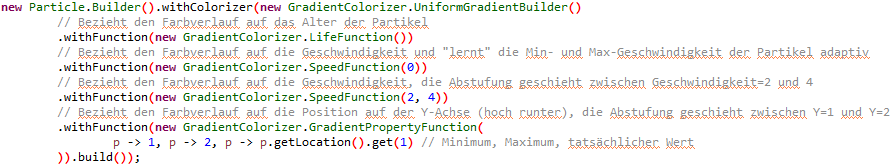
\includegraphics[width=38em]{img/gradientcolorizer_builder.png}
		\caption{GradientColorizer in einem Particle.Builder mit unterschiedlichen Funktionen (in Wirklichkeit kann immer nur eine Funktion eingesetzt werden).}
		\label{gradientcolorizer_builder}
	\end{center}
\end{figure}

\section{Konzept des ParticleColorizers f�r andere Eigenschaften}
\textmd{Das Konzept des ParticleColorizers k�nnte auch auf andere Eigenschaften als die Farbe �bertragen werden. W�hrend die Bewegung von Partikeln derzeit nur durch Einwirkung �u�erer Kr�fte umgesetzt wird, k�nnte dieses Konzept neue Bewegungsmuster erm�glichen. Vorstellbar w�ren zum Beispiel Staubpartikel die zuf�llig ihre Richtung wechseln, oder Partikel die �ber die Zeit an Masse verlieren. Dieses Konzept erm�glicht also das Ver�ndern von Eigenschaften von Partikeln �ber ihren Lebenszyklus hinweg.}

	
	%% appendix if used
	%%\appendix
	%%\typeout{===== File: appendix}
	%%\include{appendix}
	
	% bibliography and other stuff
	\backmatter
	
	\typeout{===== Section: literature}
	%% read the documentation for customizing the style
	\bibliographystyle{dinat}
	\bibliography{quellen}
	
	\typeout{===== Section: nomenclature}
	%% uncomment if a TOC entry is needed
	%%\addcontentsline{toc}{chapter}{Glossar}
	\renewcommand{\nomname}{Glossar}
	\clearpage
	\markboth{\nomname}{\nomname} %% see nomencl doc, page 9, section 4.1
	\printnomenclature
	
	%% index
	\typeout{===== Section: index}
	\printindex
	
	\HAWasurency
	
\end{document}
